\section*{Задание}
\addcontentsline{toc}{section}{Задание}

Разработать клиент-серверное приложение "Морской бой". Играют двое
пользователей-людей, обмениваясь стандартными фразами: "а7", "мимо", "ранил",
"убил". Подобный протокол взаимодействия (но на формальном уровне) должно
реализовывать сетевое приложение в режиме клиент-сервер (серверная сторона
ожидает первого хода в ее сторону). Диалог игроков-людей должен вестись в единой
кодировке (латиница или кириллица).

\newpage

\section*{Описание структуры программы}
\addcontentsline{toc}{section}{Описание структуры программы}

Проект состоит из 2 независимых программ: клиента и сервера.
Однако, они почти не отличаются друг от друга, за исключением очередности ходов.
Поэтому такое взаимодействие можно назвать одноранговым.

Подключение к серверу производится с помощью сокетов, при чем сервер блокируется
после соединения хотя бы с одним клиентом. После окончания игры сервер ожидает
подключения следующих клиентов.

Игровая часть состоит из поля размером 10х10 с клетками, которые могут
находиться в 3 состояниях:

\begin{itemize}
    \item пусто
    \item содержит целую часть корабля
    \item содержит уничтоженную часть корабля
\end{itemize}

При старте клиента или при появлении нового соединения на сервере, генерируется
новое игровое поле. Всего на нем размещается 6 кораблей размерами от 4 до 1 клеток.

Когда проверяется клетка на наличие корабля, проверяется также и 8 клеток вокруг
нее, так как полноценный корабль со всех сторон окружен пустыми клетками. Если
все соседи - не целый корабль, то возвращается сообщение о том, что корабль
полностью уничтожен. Если не осталось ни одного корабля, то вернется сообщение,
что другой пользователь проиграл.

При передаче пользователю права хода, ему предлагается ввести одну из 3 команд:
\texttt{dsp, msl, exit} - отобразить его игровое поле, <<выстрелить>> по полю
противника и выйти из сессии. Команды делятся на 2 вида: блокирующие и
неблокирующие, например команда \texttt{dsp} неблокирующая и не передает ход
оппоненту.

Поведение клиента отличается тем, что он после подключения сразу же ожидает
команды от сервера, эмулируя тем самым то, что пользователь с сервера ходит первым.

\newpage

\section*{Описание используемого протокола}
\addcontentsline{toc}{section}{Описание используемого протокола}

В программе используется собственный протокол для передачи информации об игре.
Он использует tcp-протокол сетевого уровня. Используется следующий набор
команд:

\begin{itemize}
    \item \texttt{msl <x> <y>} - <<выстрелить>> в поле противника по координатам
          \emph{x, y}. В ответ присылается \texttt{rst <code>}, где \emph{code}
          - число, показывающий попал, промазал, частично попал или проиграл ли игрок.
\end{itemize}

Для примера ниже приведена диаграмма взаимодействия клиента и сервера. Так,
клиент подключается к уже работающему серверу и они обмениваются командами
\texttt{msl}, после чего клиент отключается.

\begin{figure}[H]
    \centering
    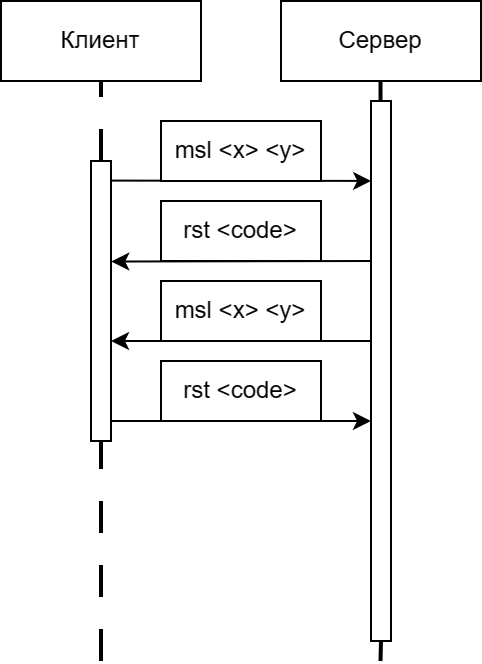
\includegraphics[width=0.4\linewidth]{images/lab3_sequence.drawio.png}
    \caption{Временная диаграмма используемого протокола}
    \label{fig:sequence}
\end{figure}

\newpage

\section*{Блок-схема программы}
\addcontentsline{toc}{section}{Блок-схема программы}

\begin{figure}[H]
    \centering
    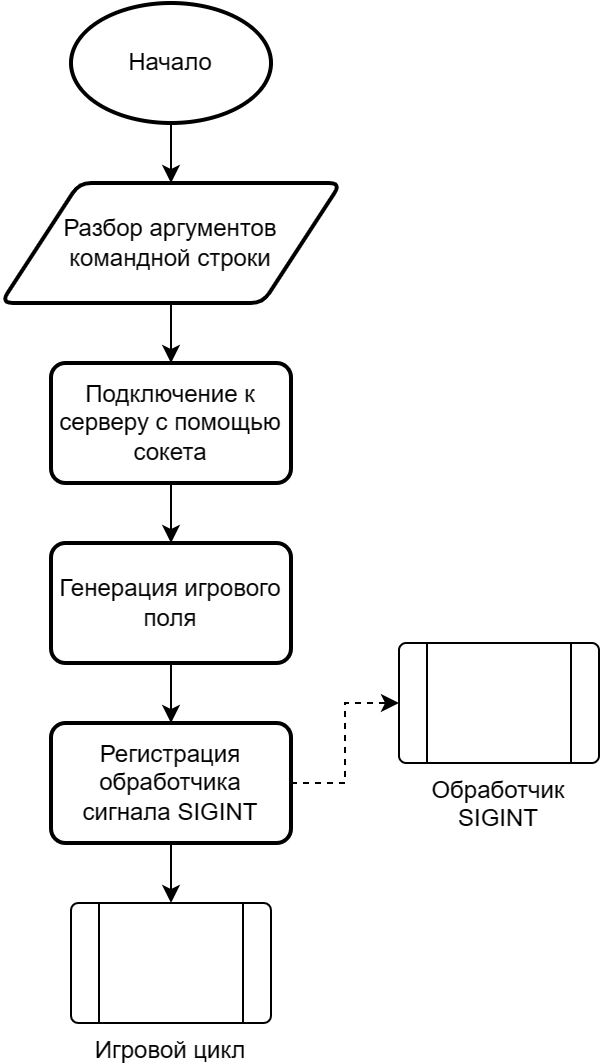
\includegraphics[width=0.5\linewidth]{images/lab3_flowchart.drawio.png}
    \caption{Основная блок-схема клиента и сервера}
    \label{fig:flowchart}
\end{figure}

\begin{figure}[H]
    \centering
    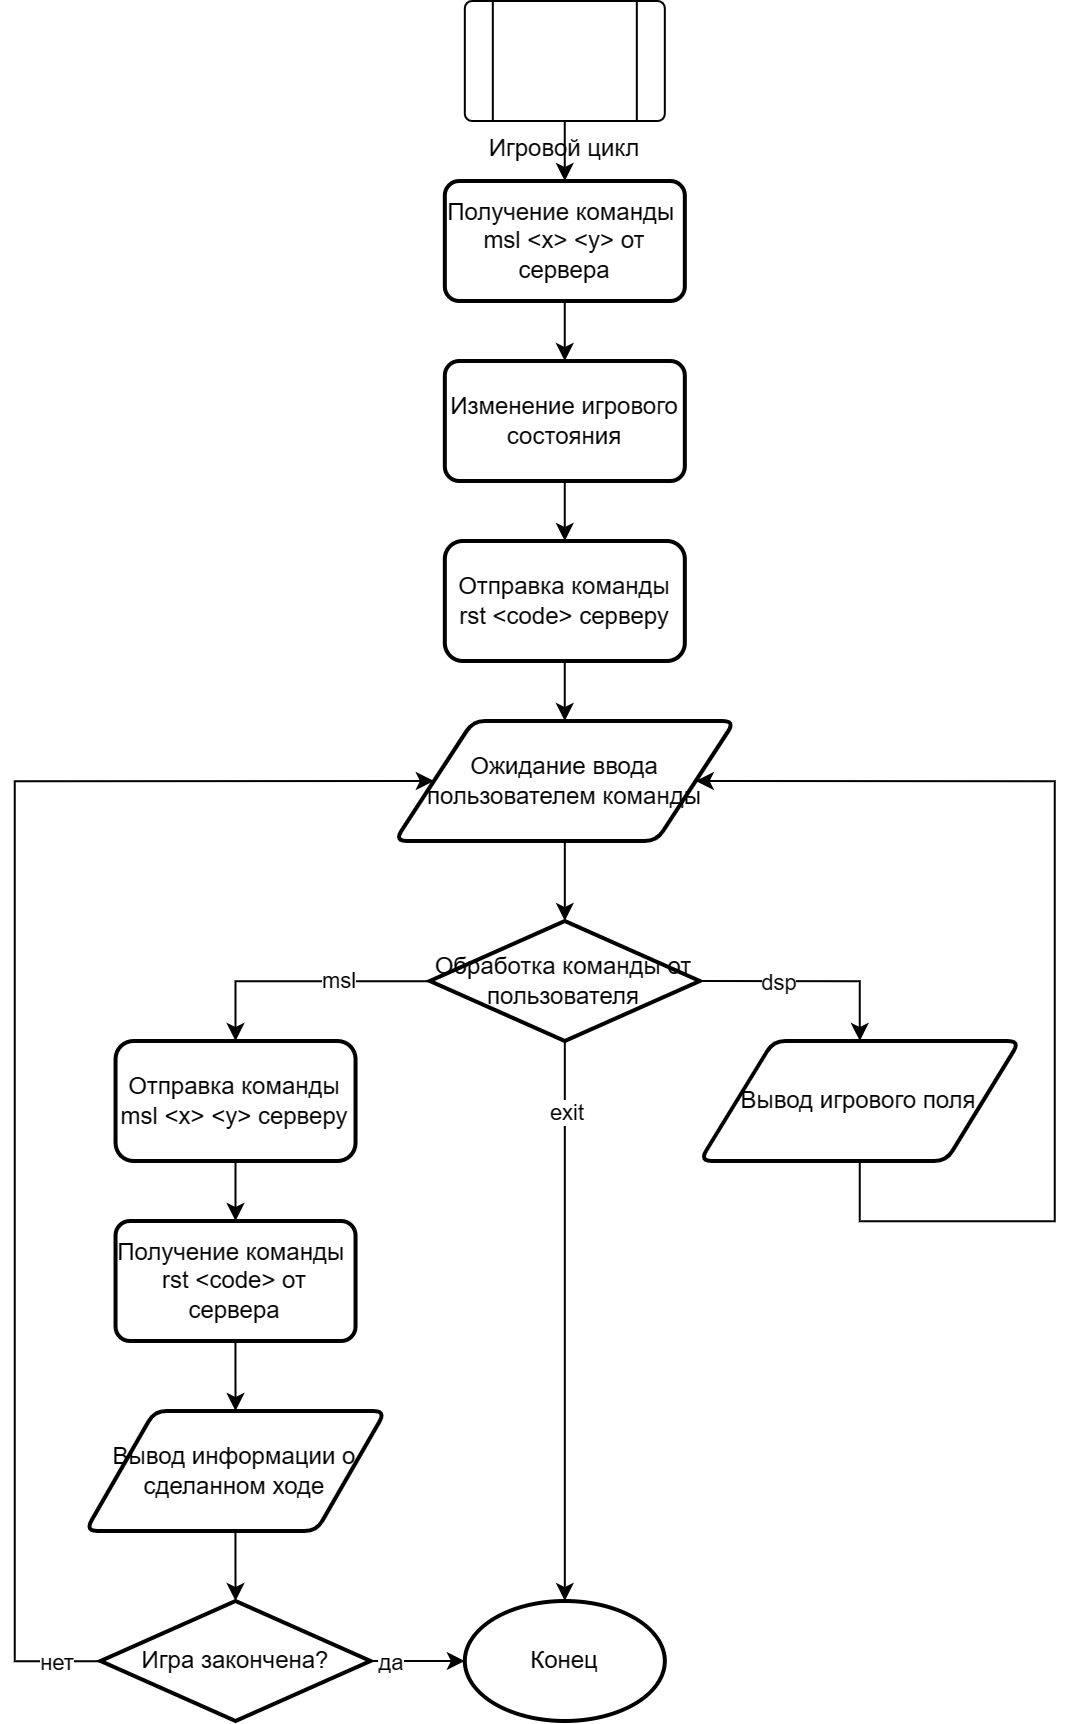
\includegraphics[width=0.85\linewidth]{images/lab3_flowchart_cont.drawio.png}
    \caption{Блок-схема части клиента}
    \label{fig:client_flowchart}
\end{figure}

\begin{figure}[H]
    \centering
    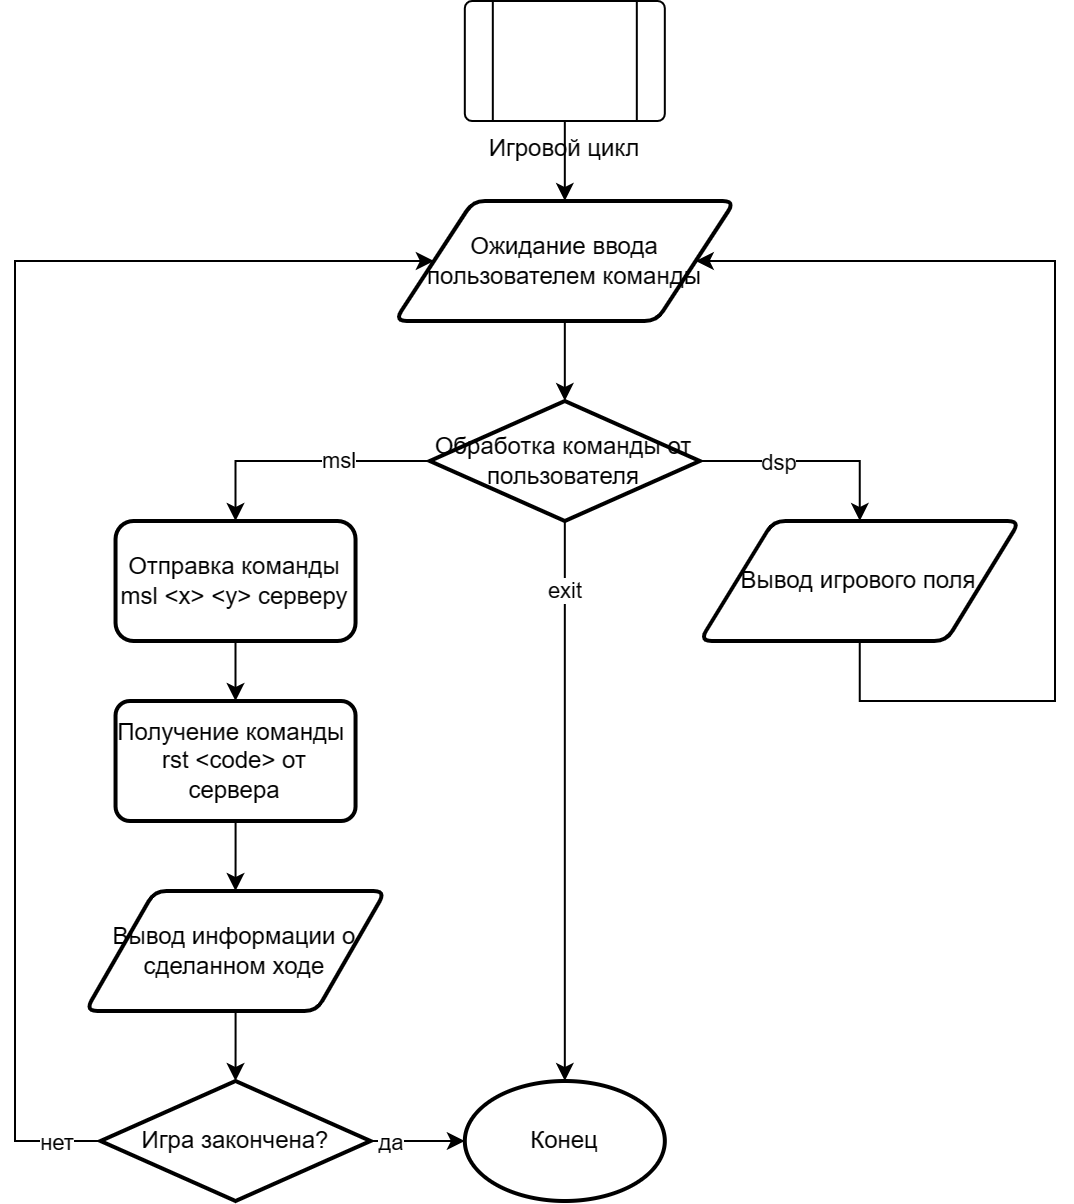
\includegraphics[width=0.85\linewidth]{images/lab3_flowchart_server.drawio.png}
    \caption{Блок-схема части сервера}
    \label{fig:server_flowchart}
\end{figure}

\begin{figure}[H]
    \centering
    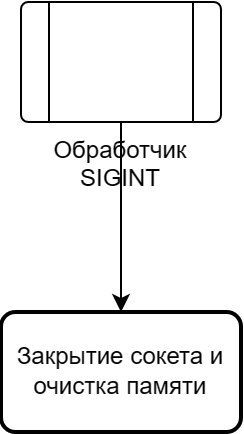
\includegraphics[width=0.2\linewidth]{images/lab3_flowchart_cont2.drawio.png}
    \caption{Блок-схема обработчика сигнала SIGINT}
    \label{fig:flowchart_sigint}
\end{figure}

\newpage

\section*{Результат работы}
\addcontentsline{toc}{section}{Результат работы}

Ниже приведены выводы программы в разные моменты времени, так как программа
меняет его в течении времени.

\begin{figure}[H]
    \centering
    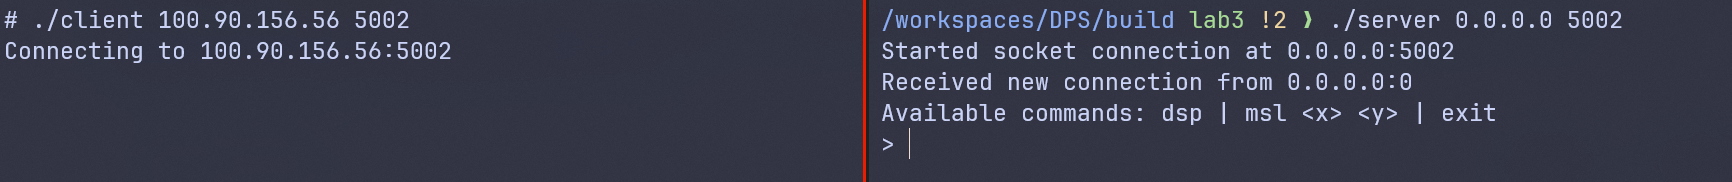
\includegraphics[width=0.9\linewidth]{images/lab3_connect.png}
    \caption{Вывод клиента и сервера при подключении клиента, где слева - вывод клиента, а справа - вывод сервера}
    \label{fig:connection}
\end{figure}

\begin{figure}[H]
    \centering
    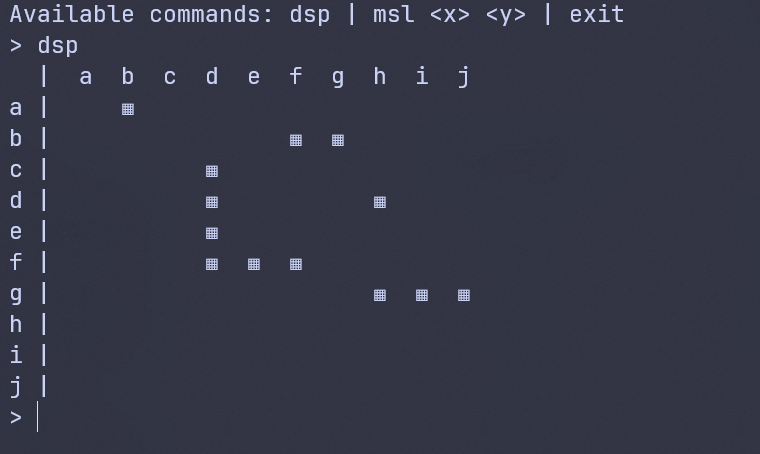
\includegraphics[width=0.5\linewidth]{images/lab3_dsp.png}
    \caption{Вывод игрового поля сервера}
    \label{fig:dsp}
\end{figure}

\begin{figure}[H]
    \centering
    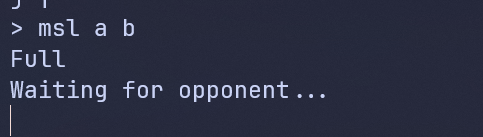
\includegraphics[width=0.3\linewidth]{images/lab3_msl.png}
    \caption{Вывод при <<выстреле>> по игровому полю противника с полным попаданием по кораблю}
    \label{fig:msl}
\end{figure}

\newpage

\appendix

\section*{Приложение}
\section*{Текст программы}
\addcontentsline{toc}{section}{Текст программы}

\textbf{include/command.h}

\begin{lstlisting}[
    language=C++,
    directivestyle={\color{black}}, 
    emph={int,char,double,float,unsigned}, 
    emphstyle={\color{blue}}]
#pragma once

#include <game.h>

/// Command types that user used to interact with program
typedef enum { Display, MissleAt, Quit, MissleRes } CommandType;

/// Contains coordinates to missle to
typedef struct {
    int x, y;
} MissleAtAttr;

/// Contain parsed command and its attributes
typedef struct {
    union {
        MissleAtAttr missle_at;
        Result missle_res;
    };

    CommandType type;
} Command;

/// Prints greet message and all allowed command to enter
void greetings();

/// Waits for user input and parses it to command object
Command ask_user();

/// Determines whether command will block execution of app until response is
/// received
bool is_blocking(Command cmd);
\end{lstlisting}

\textbf{include/game.h}

\begin{lstlisting}[
    language=C++,
    directivestyle={\color{black}}, 
    emph={int,char,double,float,unsigned}, 
    emphstyle={\color{blue}}]
#pragma once

#include <stdbool.h>

#define Size 10

/// Direction where ship is growing when map generated
typedef enum { Up, Down, Right, Left, DSize } Direction;

/// State of each cell on the game map
typedef enum { Empty = 0, Alive = 1, Dead = 2 } CellState;

/// Result of sending missle to the particular cell of the game map
typedef enum { Miss = 0, Partial = 1, Full = 2, Loose = 3 } Result;

/// Contains coordinates to 2D point of the map
typedef struct {
    int x, y;
} Point;

typedef CellState Map[Size][Size];

/// Contains game map
typedef struct {
    Map map;
} Game;

/// Fulfills game map with 6 ships
Game *generate_map();

/// Outputs current state of the game map to stdout
void display_map(Game *game);

/// Returns current cell state at specific point on the game map
CellState check_at(Game *game, Point at);

/// Checks if cell is alive at specific coords, makes it dead and returns a
/// result depending on its neighbours
Result try_kill(Game *game, Point at);
\end{lstlisting}

\textbf{include/shared.h}

\begin{lstlisting}[
    language=C++,
    directivestyle={\color{black}}, 
    emph={int,char,double,float,unsigned}, 
    emphstyle={\color{blue}}]
#pragma once

#include "command.h"
#include "game.h"
#include "socket.h"

/// Prints how to use this app to stdout
void help_prompt(const char *exec);

/// Parses ip address and port to connect to from command line args
void parse_command_args(int argc, char **argv, char **ip, unsigned short *port);

/// Applies specific command to the current game state
int process_command(Command cmd, Game *game, sock_handle socket);

/// Blocks until next response received and processes it
int receive_command(Game *game, sock_handle socket);

/// Greets the user, reads next command and processes it in infinite loop
int game_loop(Game *game, sock_handle socket);
\end{lstlisting}

\textbf{include/socket.h}

\begin{lstlisting}[
    language=C++,
    directivestyle={\color{black}}, 
    emph={int,char,double,float,unsigned}, 
    emphstyle={\color{blue}}]
#pragma once

typedef unsigned short port_t;
typedef int sock_handle;
typedef int (*socket_handler)(sock_handle);

/// Packed version of ip and port
typedef struct {
    const char *addr;
    port_t port;
} IPv4;

/// Tries to open a socket connection and bind it to specific ip and port
sock_handle open_socket_at(IPv4 ip);

/// Starts to accept socket connections. On each connection, handler is called
int accept_connections(sock_handle sock, socket_handler handler);

/// Tries to connect to a socket at specific ip and port
int open_connection(sock_handle sock, IPv4 to);
\end{lstlisting}

\textbf{include/utils.h}

\begin{lstlisting}[
    language=C++,
    directivestyle={\color{black}}, 
    emph={int,char,double,float,unsigned}, 
    emphstyle={\color{blue}}]
#pragma once

#include <stdio.h>
#include <stdlib.h>

#if DEBUG
#define DEBUG_PRINT(file, format, ...) fprintf(file, format, __VA_ARGS__)
#else
#define DEBUG_PRINT(...) 0
#endif

/// Checks if pointer is not null, otherwise returns [default] value and prints debug message to stderr (in debug mode
/// only)
#define RETURN_DEFAULT_IF_NULL(ptr, default)                                                                           \
    if ((ptr) == NULL) {                                                                                               \
        DEBUG_PRINT(stderr, "DEBUG: %s was NULL at %s:%d\n", #ptr, __FILE__, __LINE__);                                \
        return (default);                                                                                              \
    }                                                                                                                  \
    0

/// Checks if expr is non-negative integer, otherwise returns [on_error] code and prints debug message to stderr (in
/// debug mode only)
#define TRY_OR_ELSE(expr, on_error)                                                                                    \
    {                                                                                                                  \
        int code = expr;                                                                                               \
        if ((code) < 0) {                                                                                              \
            DEBUG_PRINT(stderr, "DEBUG: %s was lead to error %d at %s:%d\n", #expr, code, __FILE__, __LINE__);           \
            return on_error;                                                                                           \
        }                                                                                                              \
    }                                                                                                                  \
    0

/// Checks if expr is non-negative integer, otherwise forwards its error return code and prints debug message to stderr
/// (in debug mode only)
#define TRY_FORWARD(expr)                                                                                              \
    {                                                                                                                  \
        int code = expr;                                                                                               \
        if ((code) < 0) {                                                                                              \
            DEBUG_PRINT(stderr, "DEBUG: %s was lead to error %d at %s:%d\n", #expr, code, __FILE__, __LINE__);           \
            return code;                                                                                               \
        }                                                                                                              \
    }                                                                                                                  \
    0

/// Used in macro overloading
#define __TRY_OVERLOAD(_1, _2, name, ...) name

/// Checks if expr is non-negative integer, otherwise does action based on overload
/// SEE ALSO: [TRY_OR_ELSE], [TRY_FORWARD]
#define TRY(...) __TRY_OVERLOAD(__VA_ARGS__, TRY_OR_ELSE, TRY_FORWARD)(__VA_ARGS__)

/// Shortcut for write(..., <string literal>, sizeof(<same string literal>))
#define WRITE(fmt, message) write((fmt), (message), sizeof(message))

/// Shortcut for sizeof(<array type>) / sizeof(<type of item of array type>)
#define ARRAY_LEN(array) (sizeof(array) / sizeof(*(array)))
\end{lstlisting}

\textbf{src/client.c}

\begin{lstlisting}[
    language=C++,
    directivestyle={\color{black}}, 
    emph={int,char,double,float,unsigned}, 
    emphstyle={\color{blue}}]
#include <signal.h>
#include <sys/socket.h>
#include <time.h>
#include <unistd.h>

#include "game.h"
#include "shared.h"
#include "socket.h"
#include "utils.h"

Game *client_game;
sock_handle client_socket;

/// Called when SIGINT received. Closes opened socket connection and frees
/// memory
void graceful_shutdown(int _sig) {
    free(client_game);
    close(client_socket);
    exit(0);
}

int main(int argc, char **argv) {
    srand(time(NULL));
    char *ip;
    unsigned short port;

    parse_command_args(argc, argv, &ip, &port);
    client_socket = socket(AF_INET, SOCK_STREAM, 0);
    TRY(client_socket);

    IPv4 ip_addr = {.addr = ip, .port = port};
    printf("Connecting to %s:%d\n", ip, port);
    TRY(open_connection(client_socket, ip_addr));

    client_game = generate_map();
    signal(SIGINT, graceful_shutdown);

    TRY(receive_command(client_game, client_socket));

    greetings();

    TRY(game_loop(client_game, client_socket));
}
\end{lstlisting}

\textbf{src/command.c}

\begin{lstlisting}[
    language=C++,
    directivestyle={\color{black}}, 
    emph={int,char,double,float,unsigned}, 
    emphstyle={\color{blue}}]
#include <stdio.h>
#include <string.h>
#include <unistd.h>

#include "command.h"

void greetings() { printf("Available commands: dsp | msl <x> <y> | exit\n"); }

static void read_line(char *s) {
    char c;
    int index = 0;
    while (scanf("%c", &c) == 1) {
        if (c == EOF || c == '\n')
            break;

        s[index++] = c;
    }

    s[index] = '\0';
}

Command ask_user() {
    printf("> ");

    char x, y;
    char cmd[32];

    read_line(cmd);

    if (strncmp(cmd, "dsp", 3) == 0) {
        Command command = {.type = Display};
        return command;
    }
    if (sscanf(cmd, "msl %c %c", &x, &y) == 2) {
        MissleAtAttr attr = {.x = x - 'a', .y = y - 'a'};
        Command command = {.type = MissleAt, .missle_at = attr};
        return command;
    }
    if (strncmp(cmd, "exit", 4) == 0) {
        Command command = {.type = Quit};
        return command;
    }

    printf("Unknown command entered: %s\n", cmd);
    return ask_user();
}

bool is_blocking(Command cmd) {
    if (cmd.type == MissleAt)
        return true;
    return false;
}
\end{lstlisting}

\textbf{src/game.c}

\begin{lstlisting}[
    language=C++,
    directivestyle={\color{black}}, 
    emph={int,char,double,float,unsigned}, 
    emphstyle={\color{blue}}]
#include <stdio.h>
#include <stdlib.h>

#include "game.h"

/// Tries to make cells with start at specific coord and direction filled. Also
/// checks overlaps. Returns true if cell was populated
static bool try_place_ship(Map map, Point at, int size, Direction dir) {
    for (int i = 0; i < size; i++) {
        if (dir == Up && (at.x + i > Size || map[at.x + i][at.y]))
            return false;
        if (dir == Down && (at.x - i < 0 || map[at.x - i][at.y]))
            return false;
        if (dir == Right && (at.y + i > Size || map[at.x][at.y + i]))
            return false;
        if (dir == Left && (at.y - i < 0 || map[at.x][at.y - i]))
            return false;
    }

    for (int i = 0; i < size; i++) {
        if (dir == Up)
            map[at.x + i][at.y] = Alive;
        if (dir == Down)
            map[at.x - i][at.y] = Alive;
        if (dir == Right)
            map[at.x][at.y + i] = Alive;
        if (dir == Left)
            map[at.x][at.y - i] = Alive;
    }

    return true;
}

Game *generate_map() {
    Game *g = malloc(sizeof(Game));
    int ship_sizes[] = {4, 3, 2, 2, 1, 1};

    for (int i = 0; i < sizeof(ship_sizes) / sizeof(*ship_sizes);) {
        Point p = {.x = rand() % Size, .y = rand() % Size};
        Direction dir = rand() % DSize;

        if (try_place_ship(g->map, p, ship_sizes[i], dir))
            i++;
    }
    return g;
}

void display_map(Game *game) {
    printf("  | ");
    for (int i = 0; i < Size; i++)
        printf(" %c ", 'a' + i);
    printf("\n");

    for (int i = 0; i < Size; i++) {
        printf("%c | ", 'a' + i);

        for (int j = 0; j < Size; j++) {
            if (game->map[i][j] == Alive)
                printf(" O ");
            else if (game->map[i][j] == Dead)
                printf(" U ");
            else
                printf("   ");
        }
        printf("\n");
    }
}

CellState check_at(Game *game, Point at) { return game->map[at.x][at.y]; }

/// Returns state of cell if coord x & y available on the map, empty cell state
/// otherwise.
static CellState checked_at(Game *game, int x, int y) {
    if (0 <= x && x < Size && 0 <= y && y <= Size)
        return game->map[x][y];
    return Empty;
}

/// Returns true if any cell on the map is populated, false otherwise
static bool ships_remained(Game *game) {
    for (int i = 0; i < Size; i++)
        for (int j = 0; j < Size; j++)
            if (game->map[i][j] == Alive)
                return true;
    return false;
}

Result try_kill(Game *game, Point at) {
    if (game->map[at.x][at.y] == Empty || game->map[at.x][at.y] == Dead)
        return Miss;

    game->map[at.x][at.y] = Dead;

    if (!ships_remained(game))
        return Loose;

    if (game->map[at.x][at.y] == Dead &&
        checked_at(game, at.x - 1, at.y - 1) != Alive &&
        checked_at(game, at.x - 1, at.y + 0) != Alive &&
        checked_at(game, at.x - 1, at.y + 1) != Alive &&
        checked_at(game, at.x + 0, at.y - 1) != Alive &&
        checked_at(game, at.x + 0, at.y + 1) != Alive &&
        checked_at(game, at.x + 1, at.y - 1) != Alive &&
        checked_at(game, at.x + 1, at.y + 0) != Alive &&
        checked_at(game, at.x + 1, at.y + 1) != Alive)
        return Full;

    return Partial;
}
\end{lstlisting}

\textbf{src/server.c}

\begin{lstlisting}[
    language=C++,
    directivestyle={\color{black}}, 
    emph={int,char,double,float,unsigned}, 
    emphstyle={\color{blue}}]
#include <arpa/inet.h>
#include <signal.h>
#include <stdio.h>
#include <string.h>
#include <sys/socket.h>
#include <sys/types.h>
#include <time.h>
#include <unistd.h>

#include "shared.h"
#include "socket.h"
#include "utils.h"

sock_handle serv_sock;
Game *server_game;

/// Called when SIGINT received. Closes opened socket connection and frees
/// memory
void graceful_shutdown(int _sig) {
    free(server_game);
    close(serv_sock);
    exit(0);
}

/// Creates game map on each connection and begins game loop
int do_game(sock_handle client_socket) {
    server_game = generate_map();

    greetings();

    TRY(game_loop(server_game, client_socket));

    return 0;
}

int main(int argc, char **argv) {
    srand(time(NULL));
    char *ip;
    unsigned short port;

    parse_command_args(argc, argv, &ip, &port);

    IPv4 ip_addr = {.addr = ip, .port = port};
    serv_sock = open_socket_at(ip_addr);
    TRY(serv_sock);

    signal(SIGINT, graceful_shutdown);

    printf("Started socket connection at %s:%d\n", ip, port);

    TRY(accept_connections(serv_sock, do_game));
}
\end{lstlisting}

\textbf{src/socket.c}

\begin{lstlisting}[
    language=C++,
    directivestyle={\color{black}}, 
    emph={int,char,double,float,unsigned}, 
    emphstyle={\color{blue}}]
#include <arpa/inet.h>
#include <stdbool.h>
#include <sys/socket.h>
#include <sys/types.h>

#include "socket.h"
#include "utils.h"

sock_handle open_socket_at(IPv4 ip) {
    int sock = socket(AF_INET, SOCK_STREAM, 0);
    TRY(sock);

    struct sockaddr_in sock_addr = {.sin_family = AF_INET,
                                    .sin_port = htons(ip.port),
                                    .sin_addr = {.s_addr = inet_addr(ip.addr)}};

    TRY(bind(sock, (struct sockaddr *)&sock_addr, sizeof(sock_addr)));

    return sock;
}

int accept_connections(sock_handle sock, socket_handler handler) {
    TRY(listen(sock, 1));

    while (true) {
        struct sockaddr_in incoming;
        unsigned int incoming_size;
        sock_handle incoming_handle =
            accept(sock, (struct sockaddr *)&incoming, &incoming_size);

        TRY(incoming_handle);

        printf("Received new connection from %s:%d\n",
                inet_ntoa(incoming.sin_addr), ntohs(incoming.sin_port));
        fflush(stdout);

        handler(incoming_handle);

        printf("Client disconnected\n");
    }
}

int open_connection(sock_handle sock, IPv4 to) {
    struct sockaddr_in sock_addr = {.sin_family = AF_INET,
                                    .sin_port = htons(to.port),
                                    .sin_addr = {.s_addr = inet_addr(to.addr)}};

    TRY(connect(sock, (struct sockaddr *)&sock_addr, sizeof(sock_addr)));

    return 0;
}
\end{lstlisting}